\chapter{Applikasjon}

Dette kapittelet tar for seg arbeidsgangen i prosjektet, en detaljert arkitekturskisse, og en gjennomgang av all funksjonalitet knyttet til geoprosessering, filbehandling, grensesnitt og brukerveiledning.

\section{Arbeidsgang}

Det første som ble gjort i forbindelse med applikasjonen var å få en forståelse av hva som har blitt gjort tidligere, med tanke på valg av grensesnitt og funksjonalitet. Dette var også med på å få en forståelse av hva som var forventet og hva som ligger i ordene \textit{viktig GIS-funksjonalitet}. Et dokument som inneholdt geoprosseseringsfunksjonalitet og lagbehandlingsfunksjoner ble laget utifra tilgjengelige prosjekter\cite{Johanessen}\cite{Strand}\cite{Eglaaen}\cite{Villanger}\cite{Jakobsen} som lå tilgengelig på nett.

De ulike geoprosesseringsoperasjonene inkluderte blant annet:

\begin{frame}

    \begin{tabular}{p{0.4\textwidth}p{0.5\textwidth}}

        \begin{itemize}
            \item Clip
            \item Buffer
            \item Union
            \item Dissolve
        \end{itemize} &

        \begin{itemize}
            \item Difference
            \item Intersection
            \item Bounding box
            \item Filtering
        \end{itemize}
    \end{tabular}

\end{frame}

Mens typiske lagbehandlingsfunksjoner var:

\begin{frame}

    \begin{tabular}{p{0.4\textwidth}p{0.5\textwidth}}

        \begin{itemize}
            \item Legge til lag
            \item Fjerne lag
            \item Endre navn på lag
            \item Endre farge på navn
        \end{itemize} &

        \begin{itemize}
            \item Vise/skjule lag
            \item Zoome til lag
            \item Laste ned lag
        \end{itemize}
    \end{tabular}

\end{frame}

Etter å ha sjekket at de programmeringsspråkene jeg ønsket å jobbe med hadde støtte for denne typen operasjoner var neste steg å sette opp klient-prosjektet og server-prosjektet. Versjonskontrollsystemet git gir stor fleksibilitet til å prøve og feile, samt holde tidligere versjoner av programmet enkelt tilgjengelig hvis det skulle bli nødvendig å gå tilbake. Begge prosjektene ble knyttet til github, og kildekoden finnes på følgende nettadresser:

\href{https://github.com/torsol/PiG-frontend}{Klient-prosjektet}

\href{https://github.com/torsol/PiG-backend}{Server-prosjektet}

Den neste oppgaven var å få en minimal versjon av klient-programmet til å fungere. Det ble laget et initielt React-program som lastet inn en mapbox-komponent. Se figur \ref{fig:firstmap}. Dette var slik applikasjonen så ut etter den commiten til github 3. september. 

\begin{figure}[h]
    \center
    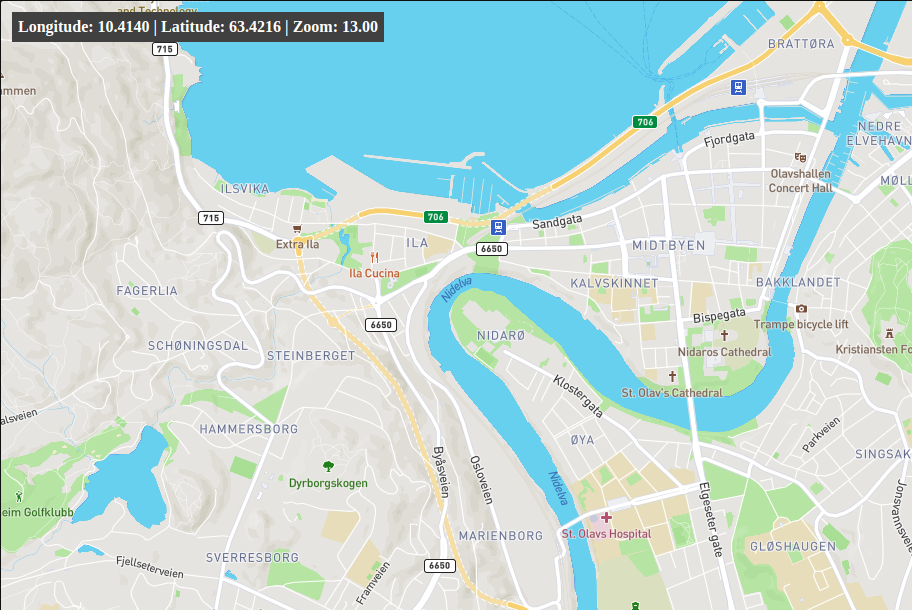
\includegraphics[scale=0.3]{first_frontend.png}
    \caption{Første versjon av klienten}
    \label{fig:firstmap}
\end{figure}

Den neste oppgaven var å få opp Server-prosjektet. Det ble gjort et bevvist valg om å holde programkodene adskilt siden de to applikasjonene i teorien kunne utvikles parallelt. Den aller første kommunikasjonen var et enkelt get-kall til flask-serveren. Som et proof of concept ville et get-kall til '/api/ping' returnere 'pong', see figure \ref{fig:firstping}. Kallet ble gjort via applikasjonen Postman, som er et utviklingsvertkøy for å foreta seg http-kall, dette ble flittig brukt for å teste ulike http-post-kall til serveren gjennom utviklingsprosessen.  

\begin{figure}[h]
    \center
    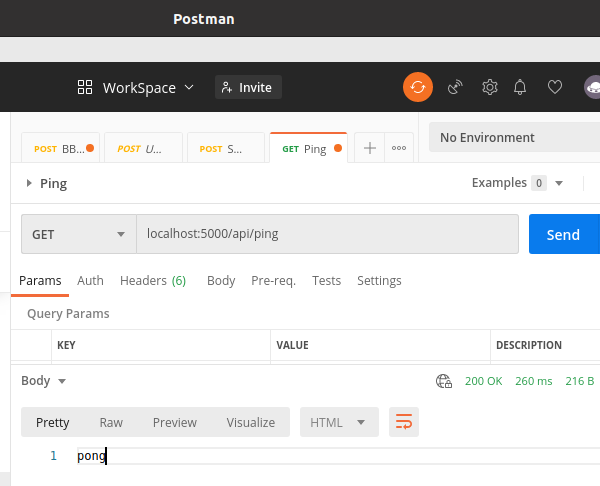
\includegraphics[scale=0.5]{ping.png}
    \caption{Første ping-pong-svar fra server, gjort via Postman}
    \label{fig:firstping}
\end{figure}

Etter at begge prosjektene var oppe og de ulike rammeverkene fungerte isolert, var hovedfokuset på å knytte sammen klient og server, ved å implementere at klienten kunne gjøre egne HTTP-kall for å få data fra serveren. Når også dette fungerte ble det satt opp en løype for å hoste de to tjenestene på github-pages og heroku, slik at man enkelt kunne gjøre nye oppdateringer i applikasjonene tilgjengelig over nett. Mer om dette kommer i seksjon \ref{sec:hosting}.

Når hovedarkitekturen var på plass flyttet fokuset seg over til å implementere mer funksjonalitet og brukergrensesnitt. Funksjonalitet var drevet av de kartlagte funksjonene funnet tidligere i arbeidsprosessen, mens brukergrensesnittet ble laget inspirert av målene om at applikasjonen skulle være brukervennlig og at det skulle bestå av mest mulig interaksjon i kartet. 

Videre ble det forberedt data og laget en brukerveiledning som kan finnes både inne i klienten, men også i denne rapporten i appendiks \ref{sec:brukerveiledning}. Helt tilslutt gjenstod det å oppsummere arbeidet i denne rapportne og lansere den endelige versjonen. 

\section{Detaljert arkitektur}

- Design principles

\section{Funksonalitet}

\subsection{Brukergrensesnitt}

- Tilbakemelding på feil eller suksess

- Design

- Minst mulig sidemenyer

- Kartdesign

\subsection{Geoprosessering}

\subsection{Lagbehandling}

\subsection{Brukerveiledning}

\section{Hosting}
\label{sec:hosting}
